\section{Methods for sentiment classification}
\label{sec:class}

Our goal is to use our unbiased sample of the Twitter user population
to infer the sentiment of the Twitter population over time. We define our
classification problem as follows: given a collection of tweets, classify each
as having positive, neutral, or negative sentiment. We explored a variety of
unsupervised and supervised learning methods. 

\subsection{Unsupervised}

We apply two clustering techniques to put tweets into three groups positive, neutral, and negative.

\paragraph{KMeans}

KMeans creates clusters out of the means of the features. Twitter
tweets have few words and no shared topic, making our unigram-based
feature vectors very sparse. This makes it difficult to apply Kmeans.
We performed dimension reduction with Principal Component Analysis
(PCA) to try to mitigate this problem. Figure~\ref{fig:pca} shows the makeup
of the top four components. Although the PCA components seem to
reflect some sentimental words, it does not distinguish the words by
sentiments very well. The very short length of a tweet makes it unlikely
that two positive words will appear together, thereby preventing
correlation between words of the same sentiment.

\begin{figure*}[htb]
\begin{center}
  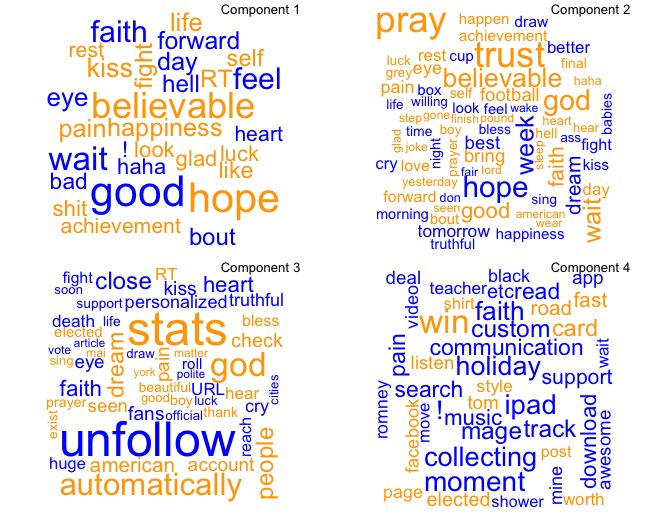
\includegraphics[width=0.8\linewidth]{figs/PCAcomp.png}
\begin{minipage}{0.8\linewidth}
\end{minipage}
\end{center}
\caption{Four principal components from the word features of the labeled dataset. Within each component blue words differentiated positive and orange words differentiated negative.}
\label{fig:pca}
\end{figure*}


\paragraph{Naive bayes with word polarity}

A domain-specific alternative to structure-based dimension reduction
is rating word features by sentiment, thus collapsing sparse vectors
of word features into polarities. We assign a weight
based on some prior probability of a word being positive or negative.
Many datasets exist with such information. Data can be in the form of
positive/negative word lists \cite{MPQA,BingLiu} or as an ordinal
rating \cite{MPQA}. We trained a naive Bayes classifier on the
Multi-perspective question answering subjectivity lexicon~\cite{MPQA}.
Applying naive Bayes requires the assumption that the features are
independent. To classify, naive bayes calculates the likelihood that
tweet a tweet has a particular sentiment.
\begin{align}
    Pr(+|tweet) &\propto Pr(tweet|+)Pr(+) \\
    &\propto \prod_{word \in tweet} Pr(word|+)Pr(+)
\end{align}
The $Pr(word|sentiment)$ come from the lexicon data for each word.
We could similarly apply this method to a multi-valued positivity
rating, such as the IMDB ratings dataset. This dataset contains a
rating distribution for each word based on movie reviews it appears in
(example in Figure~\ref{fig:imdb-word}). We pick rating decision
boundaries to divide the three classes of tweets.
Figure~\ref{fig:imdb-mean} shows the mean probability distribution of
ratings in each sentiment class.
A limitation of this approach is that it involves the assumption that
the prior on word sentiment for tweets is the same as that of the word rating
data source. The difference in priors between this dataset and ours
could skew the result. The IMDB dataset has a heavy tail of high
ratings: of 317 million reviews, 23.3\% have rating 10 and 12.7\% have
rating 9, while we do not expect the same in tweets.

\begin{figure}[htb]
\begin{center}
  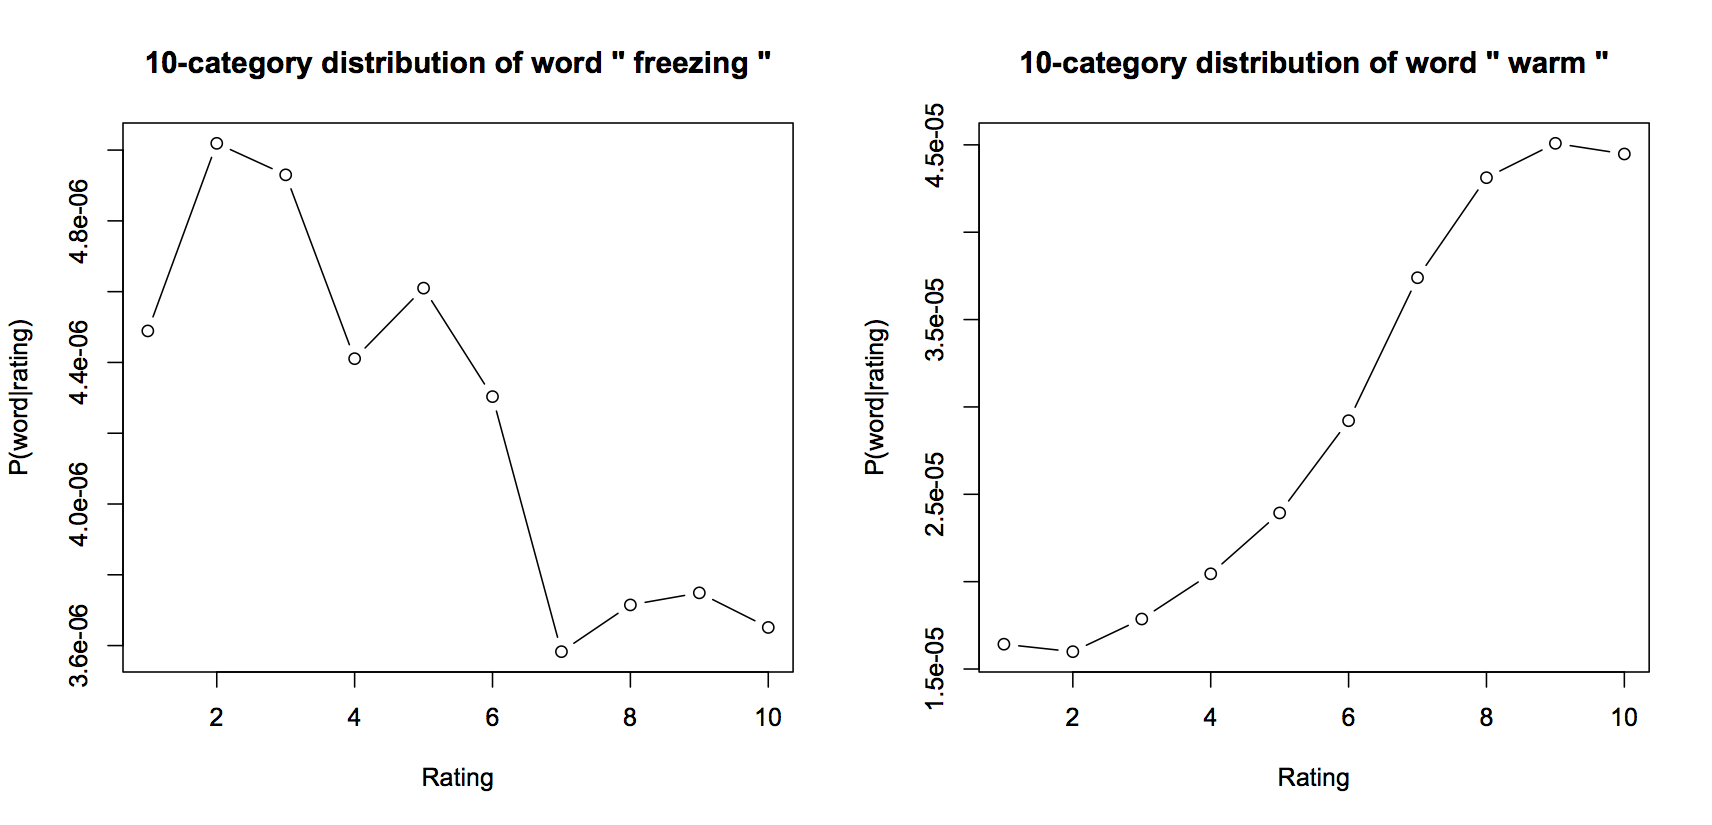
\includegraphics[width=0.9\columnwidth]{figs/wordIMDB.png}
\begin{minipage}{0.9\columnwidth}
\end{minipage}
\end{center}
\caption{Example: probability of a word appearing in documents of
    various ratings}
\label{fig:imdb-word}
\end{figure}


\begin{figure*}[htb]
\begin{center}
  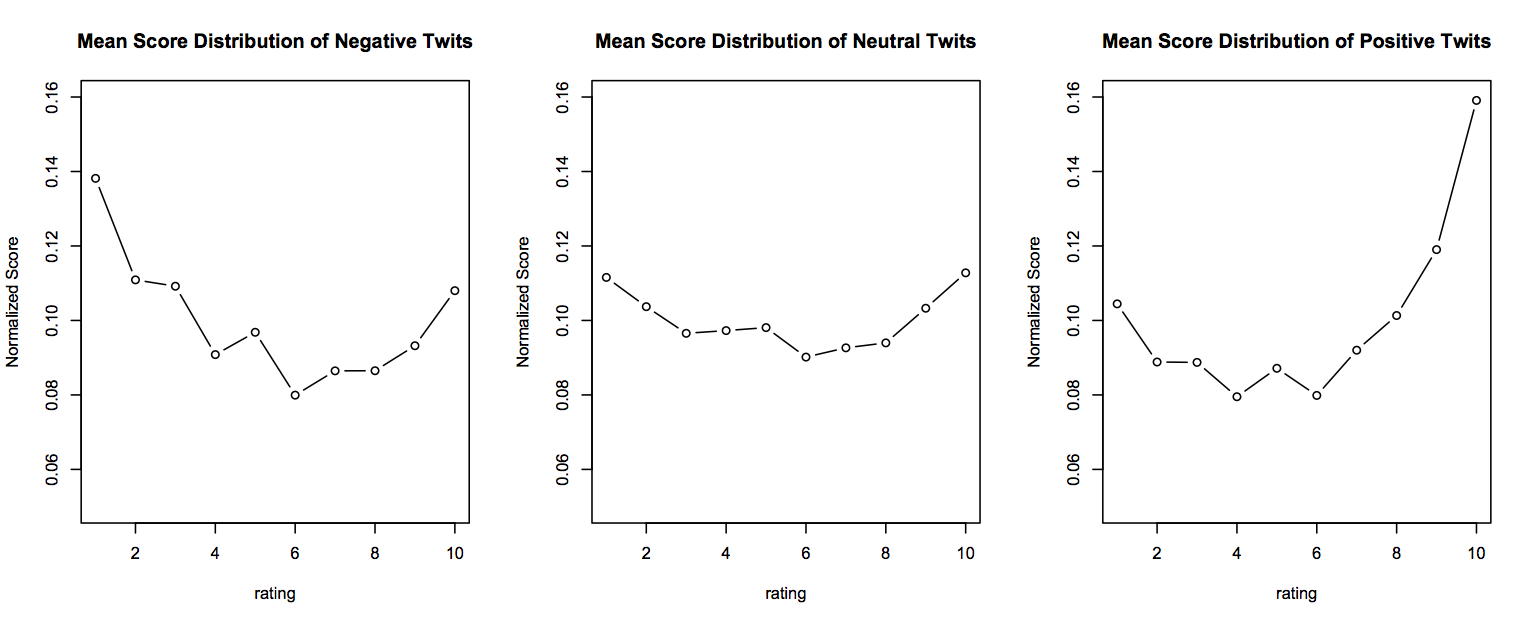
\includegraphics[width=0.9\linewidth]{figs/meanIMDB.png}
\begin{minipage}{0.9\linewidth}
\end{minipage}
\end{center}
\caption{Mean probability distribution of ratings in each sentiment
    class}
\label{fig:imdb-mean}
\end{figure*}


\subsection{Supervised}

Using our labeled dataset, we applied four supervised learning
techniques: Naive Bayes classifier, Linear Discriminant Analysis
(LDA), Support Vector Machine (SVM), K Nearest Neighbors (KNN). All
have been used in text classification efforts and have different
advantages when applied to Twitter sentiment.

\paragraph{Naive Bayes classifier}

This technique is the most simple because of its strong independence
assumptions, and it is often used as a baseline when comparing
accuracy of text classification. Other work has shown it to have
comparable accuracy as more sophisticated classifiers in the domain of
Twitter tweets~\cite{Pak:2010}. We find that Naive Bayes performs
relatively poorly on our data because our labeled training set is too small to
overcome the sparse feature space.

\paragraph{Support Vector Machine}

Training an SVM creates a hyperplane that maximizes the margin between
two classes. When there are multiple classes, as in our case of 3
sentiment levels, we run SVM on pairs of classes and use voting to
determine the label. We tried a linear kernel and Gaussian radial
kernel to fit a model and found gaussian to have slightly better
accuracy.

\paragraph{Linear Discriminant Analysis}

This is another technique that is often used in text classification.
It is similar to an SVM with a linear kernel but LDA finds the best
combination of features to separate the classes.

\paragraph{K Nearest Neighbors}

Unlike the other supervised methods that rely on calculating a closed formula for
the decision boundary, the borders provided by KNN are implicit and
determined by similar data points. For our problem, a design space
search on $K \in [1,50]$ found that K=5 gives best accuracy.





